%
% This is an example LaTeX file which uses the SANDreport class file.
% It shows how a SAND report should be formatted, what sections and
% elements it should contain, and how to use the SANDreport class.
% It uses the LaTeX article class, but not the strict option.
% ItINLreport uses .eps logos and files to show how pdflatex can be used
%
% Get the latest version of the class file and more at
%    http://www.cs.sandia.gov/~rolf/SANDreport
%
% This file and the SANDreport.cls file are based on information
% contained in "Guide to Preparing {SAND} Reports", Sand98-0730, edited
% by Tamara K. Locke, and the newer "Guide to Preparing SAND Reports and
% Other Communication Products", SAND2002-2068P.
% Please send corrections and suggestions for improvements to
% Rolf Riesen, Org. 9223, MS 1110, rolf@cs.sandia.gov
%
\documentclass[pdf,12pt]{INLreport}
% pslatex is really old (1994).  It attempts to merge the times and mathptm packages.
% My opinion is that it produces a really bad looking math font.  So why are we using it?
% If you just want to change the text font, you should just \usepackage{times}.
% \usepackage{pslatex}
\usepackage{times}
\usepackage[FIGBOTCAP,normal,bf,tight]{subfigure}
\usepackage{amsmath}
\usepackage{amssymb}
\usepackage{soul}
\usepackage{pifont}
\usepackage{enumerate}
\usepackage{listings}
\usepackage{fullpage}
\usepackage{xcolor}          % Using xcolor for more robust color specification
\usepackage{ifthen}          % For simple checking in newcommand blocks
\usepackage{textcomp}
\usepackage{mathtools}
\usepackage{relsize}
\usepackage{lscape}
\usepackage[toc,page]{appendix}
\usepackage{RAVEN}

\newtheorem{mydef}{Definition}
\newcommand{\norm}[1]{\lVert#1\rVert}
%\usepackage[table,xcdraw]{xcolor}
%\usepackage{authblk}         % For making the author list look prettier
%\renewcommand\Authsep{,~\,}

% Custom colors
\definecolor{deepblue}{rgb}{0,0,0.5}
\definecolor{deepred}{rgb}{0.6,0,0}
\definecolor{deepgreen}{rgb}{0,0.5,0}
\definecolor{forestgreen}{RGB}{34,139,34}
\definecolor{orangered}{RGB}{239,134,64}
\definecolor{darkblue}{rgb}{0.0,0.0,0.6}
\definecolor{gray}{rgb}{0.4,0.4,0.4}

\lstset {
  basicstyle=\ttfamily,
  frame=single
}


\setcounter{secnumdepth}{5}
\lstdefinestyle{XML} {
    language=XML,
    extendedchars=true,
    breaklines=true,
    breakatwhitespace=true,
%    emph={name,dim,interactive,overwrite},
    emphstyle=\color{red},
    basicstyle=\ttfamily,
%    columns=fullflexible,
    commentstyle=\color{gray}\upshape,
    morestring=[b]",
    morecomment=[s]{<?}{?>},
    morecomment=[s][\color{forestgreen}]{<!--}{-->},
    keywordstyle=\color{cyan},
    stringstyle=\ttfamily\color{black},
    tagstyle=\color{darkblue}\bf\ttfamily,
    morekeywords={name,type},
%    morekeywords={name,attribute,source,variables,version,type,release,x,z,y,xlabel,ylabel,how,text,param1,param2,color,label},
}
\lstset{language=python,upquote=true}

\usepackage{titlesec}
\newcommand{\sectionbreak}{\clearpage}
\setcounter{secnumdepth}{4}

%\titleformat{\paragraph}
%{\normalfont\normalsize\bfseries}{\theparagraph}{1em}{}
%\titlespacing*{\paragraph}
%{0pt}{3.25ex plus 1ex minus .2ex}{1.5ex plus .2ex}

%%%%%%%% Begin comands definition to input python code into document
\usepackage[utf8]{inputenc}

% Default fixed font does not support bold face
\DeclareFixedFont{\ttb}{T1}{txtt}{bx}{n}{9} % for bold
\DeclareFixedFont{\ttm}{T1}{txtt}{m}{n}{9}  % for normal

\usepackage{listings}

% Python style for highlighting
\newcommand\pythonstyle{\lstset{
language=Python,
basicstyle=\ttm,
otherkeywords={self, none, return},             % Add keywords here
keywordstyle=\ttb\color{deepblue},
emph={MyClass,__init__},          % Custom highlighting
emphstyle=\ttb\color{deepred},    % Custom highlighting style
stringstyle=\color{deepgreen},
frame=tb,                         % Any extra options here
showstringspaces=false            %
}}


% Python environment
\lstnewenvironment{python}[1][]
{
\pythonstyle
\lstset{#1}
}
{}

% Python for external files
\newcommand\pythonexternal[2][]{{
\pythonstyle
\lstinputlisting[#1]{#2}}}

\lstnewenvironment{xml}
{}
{}

% Python for inline
\newcommand\pythoninline[1]{{\pythonstyle\lstinline!#1!}}

% Named Colors for the comments below (Attempted to match git symbol colors)
\definecolor{RScolor}{HTML}{8EB361}  % Sonat (adjusted for clarity)
\definecolor{DPMcolor}{HTML}{E28B8D} % Dan
\definecolor{JCcolor}{HTML}{82A8D9}  % Josh (adjusted for clarity)
\definecolor{AAcolor}{HTML}{8D7F44}  % Andrea
\definecolor{CRcolor}{HTML}{AC39CE}  % Cristian
\definecolor{RKcolor}{HTML}{3ECC8D}  % Bob (adjusted for clarity)
\definecolor{DMcolor}{HTML}{276605}  % Diego (adjusted for clarity)
\definecolor{PTcolor}{HTML}{990000}  % Paul

\def\DRAFT{} % Uncomment this if you want to see the notes people have been adding
% Comment command for developers (Should only be used under active development)
\ifdefined\DRAFT
  \newcommand{\nameLabeler}[3]{\textcolor{#2}{[[#1: #3]]}}
\else
  \newcommand{\nameLabeler}[3]{}
\fi
\newcommand{\alfoa}[1] {\nameLabeler{Andrea}{AAcolor}{#1}}
\newcommand{\cristr}[1] {\nameLabeler{Cristian}{CRcolor}{#1}}
\newcommand{\mandd}[1] {\nameLabeler{Diego}{DMcolor}{#1}}
\newcommand{\maljdan}[1] {\nameLabeler{Dan}{DPMcolor}{#1}}
\newcommand{\cogljj}[1] {\nameLabeler{Josh}{JCcolor}{#1}}
\newcommand{\bobk}[1] {\nameLabeler{Bob}{RKcolor}{#1}}
\newcommand{\senrs}[1] {\nameLabeler{Sonat}{RScolor}{#1}}
\newcommand{\talbpaul}[1] {\nameLabeler{Paul}{PTcolor}{#1}}
% Commands for making the LaTeX a bit more uniform and cleaner
\newcommand{\TODO}[1]    {\textcolor{red}{\textit{(#1)}}}
\newcommand{\xmlAttrRequired}[1] {\textcolor{red}{\textbf{\texttt{#1}}}}
\newcommand{\xmlAttr}[1] {\textcolor{cyan}{\textbf{\texttt{#1}}}}
\newcommand{\xmlNodeRequired}[1] {\textcolor{deepblue}{\textbf{\texttt{<#1>}}}}
\newcommand{\xmlNode}[1] {\textcolor{darkblue}{\textbf{\texttt{<#1>}}}}
\newcommand{\xmlString}[1] {\textcolor{black}{\textbf{\texttt{'#1'}}}}
\newcommand{\xmlDesc}[1] {\textbf{\textit{#1}}} % Maybe a misnomer, but I am
                                                % using this to detail the data
                                                % type and necessity of an XML
                                                % node or attribute,
                                                % xmlDesc = XML description
\newcommand{\default}[1]{~\\*\textit{Default: #1}}
\newcommand{\nb} {\textcolor{deepgreen}{\textbf{~Note:}}~}


%%%%%%%% End comands definition to input python code into document

%\usepackage[dvips,light,first,bottomafter]{draftcopy}
%\draftcopyName{Sample, contains no OUO}{70}
%\draftcopyName{Draft}{300}

% The bm package provides \bm for bold math fonts.  Apparently
% \boldsymbol, which I used to always use, is now considered
% obsolete.  Also, \boldsymbol doesn't even seem to work with
% the fonts used in this particular document...
\usepackage{bm}


% Define tensors to be in bold math font.
\newcommand{\tensor}[1]{{\bm{#1}}}

% Override the formatting used by \vec.  Instead of a little arrow
% over the letter, this creates a bold character.
\renewcommand{\vec}{\bm}

% Define unit vector notation.  If you don't override the
% behavior of \vec, you probably want to use the second one.
\newcommand{\unit}[1]{\hat{\bm{#1}}}
% \newcommand{\unit}[1]{\hat{#1}}

% Use this to refer to a single component of a unit vector.
\newcommand{\scalarunit}[1]{\hat{#1}}

% Aliases
\newcommand{\raven}{\texttt{RAVEN}}
\newcommand{\ravens}{\texttt{RAVEN}'s}
\newcommand{\plugin}{\raven{} Plugin}
\newcommand{\plugins}{\raven{} Plugins}


% \toprule, \midrule, \bottomrule for tables
\usepackage{booktabs}

% \llbracket, \rrbracket
\usepackage{stmaryrd}

\usepackage{hyperref}
\hypersetup{
    colorlinks,
    citecolor=black,
    filecolor=black,
    linkcolor=black,
    urlcolor=black
}

% Compress lists of citations like [33,34,35,36,37] to [33-37]
\usepackage{cite}

% If you want to relax some of the SAND98-0730 requirements, use the "relax"
% option. It adds spaces and boldface in the table of contents, and does not
% force the page layout sizes.
% e.g. \documentclass[relax,12pt]{SANDreport}
%
% You can also use the "strict" option, which applies even more of the
% SAND98-0730 guidelines. It gets rid of section numbers which are often
% useful; e.g. \documentclass[strict]{SANDreport}

% The INLreport class uses \flushbottom formatting by default (since
% it's intended to be two-sided document).  \flushbottom causes
% additional space to be inserted both before and after paragraphs so
% that no matter how much text is actually available, it fills up the
% page from top to bottom.  My feeling is that \raggedbottom looks much
% better, primarily because most people will view the report
% electronically and not in a two-sided printed format where some argue
% \raggedbottom looks worse.  If we really want to have the original
% behavior, we can comment out this line...
\raggedbottom
\setcounter{secnumdepth}{5} % show 5 levels of subsection
\setcounter{tocdepth}{5} % include 5 levels of subsection in table of contents

% ---------------------------------------------------------------------------- %
%
% Set the title, author, and date
%
\title{RAVEN Plugins Manual}
%\author{%
%\begin{tabular}{c} Author 1 \\ University1 \\ Mail1 \\ \\
%Author 3 \\ University3 \\ Mail3 \end{tabular} \and
%\begin{tabular}{c} Author 2 \\ University2 \\ Mail2 \\ \\
%Author 4 \\ University4 \\ Mail4\\
%\end{tabular} }


\author{
\\Paul W. Talbot
\\Congjian Wang
}

% There is a "Printed" date on the title page of a SAND report, so
% the generic \date should [WorkingDir:]generally be empty.
\date{}


% ---------------------------------------------------------------------------- %
% Set some things we need for SAND reports. These are mandatory
%
\SANDnum{INL/EXT-TODO}
\SANDprintDate{\today}
\SANDauthor{Paul W. Talbot, Congjian Wang}
\SANDreleaseType{Revision 0}


% ---------------------------------------------------------------------------- %
% Include the markings required for your SAND report. The default is "Unlimited
% Release". You may have to edit the file included here, or create your own
% (see the examples provided).
%
% \include{MarkOUO} % Not needed for unlimted release reports

\def\component#1{\texttt{#1}}

% ---------------------------------------------------------------------------- %
\newcommand{\systemtau}{\tensor{\tau}_{\!\text{SUPG}}}

% Added by Sonat
\usepackage{placeins}
\usepackage{array}

\newcolumntype{L}[1]{>{\raggedright\let\newline\\\arraybackslash\hspace{0pt}}m{#1}}
\newcolumntype{C}[1]{>{\centering\let\newline\\\arraybackslash\hspace{0pt}}m{#1}}
\newcolumntype{R}[1]{>{\raggedleft\let\newline\\\arraybackslash\hspace{0pt}}m{#1}}

% end added by Sonat
% ---------------------------------------------------------------------------- %
%
% Start the document
%

\begin{document}
    \sloppy
    \maketitle

    % ------------------------------------------------------------------------ %
    % An Abstract is required for SAND reports
    %
%    \begin{abstract}
%    \input abstract
%    \end{abstract}


    % ------------------------------------------------------------------------ %
    % An Acknowledgement section is optional but important, if someone made
    % contributions or helped beyond the normal part of a work assignment.
    % Use \section* since we don't want it in the table of context
    %
%    \clearpage
%    \section*{Acknowledgment}



%	The format of this report is based on information found
%	in~\cite{Sand98-0730}.


    % ------------------------------------------------------------------------ %
    % The table of contents and list of figures and tables
    % Comment out \listoffigures and \listoftables if there are no
    % figures or tables. Make sure this starts on an odd numbered page
    %
    \cleardoublepage		% TOC needs to start on an odd page
    \tableofcontents
    %\listoffigures
    %\listoftables


    % ---------------------------------------------------------------------- %
    % An optional preface or Foreword
%    \clearpage
%    \section*{Preface}
%    \addcontentsline{toc}{section}{Preface}
%	Although muggles usually have only limited experience with
%	magic, and many even dispute its existence, it is worthwhile
%	to be open minded and explore the possibilities.


    % ---------------------------------------------------------------------- %
    % An optional executive summary
    %\clearpage
    %\section*{Summary}
    %\addcontentsline{toc}{section}{Summary}
    %\input{Summary.tex}
%	Once a certain level of mistrust and skepticism has
%	been overcome, magic finds many uses in todays science



%	and engineering. In this report we explain some of the
%	fundamental spells and instruments of magic and wizardry. We
%	then conclude with a few examples on how they can be used
%	in daily activities at national Laboratories.


    % ---------------------------------------------------------------------- %
    % An optional glossary. We don't want it to be numbered
%    \clearpage
%    \section*{Nomenclature}
%    \addcontentsline{toc}{section}{Nomenclature}
%    \begin{description}
%          \item[alohomoral]
%           spell to open locked doors and containers
%          \item[leviosa]
%           spell to levitate objects
%    \item[remembrall]
%           device to alert you that you have forgotten something
%    \item[wand]
%           device to execute spells
%    \end{description}


    % ---------------------------------------------------------------------- %
    % This is where the body of the report begins; usually with an Introduction
    %
    \SANDmain		% Start the main part of the report





\label{sec:introduction}
RAVEN (\textbf{R}eactor \textbf{A}nalysis and \textbf{V}irtual control \textbf{EN}viroment)~\cite{ravenFY12,mandelliANS2012} is a software tool that acts as the control logic driver for the newly developed Thermal-Hydraulic code RELAP-7  (\textbf{R}eactor \textbf{E}xcursion and \textbf{L}eak \textbf{A}nalysis \textbf{P}rogram).
RAVEN has been designed in a highly modular and pluggable way in order to enable easy integration of different programming languages (i.e., C++, Python) and coupling with other MOOSE based and external applications.
\\The goal of this report is to highlight the newly developed  Dynamic Event Tree (DET) module embedded in the code and its utilization in conjunction with RELAP-7.

As for all \textbf{P}robabilistic \textbf{R}isk \textbf{A}ssessment (PRA) software the capability to fully control the plant evolution during the simulation represents a highly desirable feature as it is for the analysis of the propagation of the uncertainty. . For these reasons, a strict interaction between RELAP-7 and RAVEN is a key of the long-term success of the overall project. In system safety analysis codes, a similar need is expressed by the implementation of the control logic of the plant. As a consequence the optimization of resources imposes the integration of this task under a common project that is naturally RAVEN.The final outcome is a very general and flexible implementation of the plant control logic that will easily allow the integration of proprietary information without any change in the RELAP-7 code. This is also regarded as a facilitating factor for the quick deployment of RELAP-7.

In summary, RAVEN is a multi-purpose PRA software framework that allows dispatching different functionalities.
It is designed to derive and actuate the control logic required to simulate the plant control system and operator actions (guided procedures) and to perform both Monte-Carlo sampling  and Event Tree based analysis of the probabilistic behavior of the NPP.
In order to facilitate the input/output handling, a \textbf{G}raphical \textbf{U}ser \textbf{I}nterface (GUI) and a post-processing data mining module (under development) are available.

This report provides an overview of the DET structure, highlighting the mathematical framework from which its structure is derived and its software implementation. In addition a \textbf{S}tation \textbf{B}lack \textbf{O}ut (SBO) DET based analysis of a simplified \textbf{P}ressurized \textbf{W}ater \textbf{R}eactor (PWR) model will be shown.
\vspace{-5mm}

%\subsection{subsection}
%text

%figure template

%\subsubsection{subsubsection}
%more text
%\paragraph{paragraph}
%lot of text
%\subparagraph{subparagraph}
%if you arrive at this point you have issues

\section{Making a New RAVEN Plugin}

Creating a new plugin is a straightforward process. It involves setting up a repository,
establishing a basic structure, and installing in RAVEN for testing.

%\subsection{Setting up a Repository}
%TODO

\subsection{Plugin Structure}
The following directories and \texttt{\_\_init\_\_.py} must be present in the main directory of the plugin in order for RAVEN to
read it correctly as shown in figure~\ref{fig:pluginsLocation}:
\begin{itemize}
  \item \texttt{src}, where the entities for RAVEN to load are located;
  \item \texttt{doc}, where the documentation for the plugin and its entities is located.
  \item \texttt{tests}, where continuous integration tests are located;
  \item \texttt{\_\_init\_\_.py}, where the plugin entities need to be loaded.
\end{itemize}

Here is the example for \texttt{\_\_init\_\_.py} from the \texttt{raven/plugins/ExamplePlugin}:
\begin{lstlisting}[language=python, breaklines=True, columns=fullflexible]
### External Model
from ExamplePlugin.src import SumOfExponential
### ROM
from ExamplePlugin.src import LinearROM
### Outstreams
from ExamplePlugin.src import CorrelationPlot
### PostProcessors
from ExamplePlugin.src import testInterfacedPP
from ExamplePlugin.src import testInterfacedPP_PointSet
\end{lstlisting}

If the plugin developer wants to make his plugin
an official supported plugin in RAVEN (by the submodule system), he needs to check
the raven wiki under the ``contribution'' section), and this plugin needs to be placed in a folder (whatever name) located
in (see figure~\ref{fig:pluginsLocation} for example):
\begin{lstlisting}[language=bash]
 path/to/raven/plugins/
\end{lstlisting}

\begin{figure}
\centering
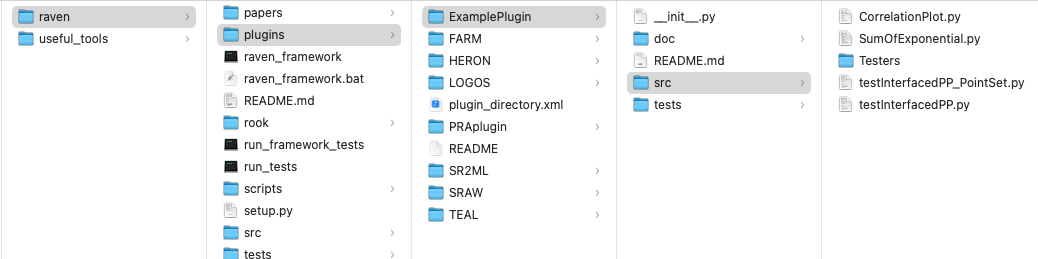
\includegraphics[width=1.0\textwidth]{pics/plugins_location.png}
\caption{Plugins Location}
\label{fig:pluginsLocation}
\end{figure}

\subsection{Plugin Entities}
The procedure of adding a plugin entity for RAVEN is a straightforward process.
The addition of the entity does not require modifying RAVEN itself.
Instead, the developer creates a new Python module inherited from plugin base class that is going to be embedded
in RAVEN at run-time (no need to introduce  hard-coded statements). These RAVEN plugin base
classes are located at \texttt{raven/ravenframework/PluginBaseClasses}:
\begin{lstlisting}[language=bash]
 ExternalModelPluginBase in ExternalModelPluginBase.py
 PlotPlugin in OutStreamPlotPlugin.py
 PostProcessorPluginBase in PostProcessorPluginBase.py
 SupervisedLearningPlugin in SupervisedLearningPlugin.py
\end{lstlisting}
These classes can be loaded as follows in the Python modules created by the plugin developers:
\begin{lstlisting}[language=python, basicstyle=\scriptsize\ttfamily, breaklines=True, columns=fullflexible]
 from ravenframework.PluginBaseClasses.ExternalModelPluginBase import ExternalModelPluginBase
 from ravenframework.PluginBaseClasses.OutStreamPlotPlugin import PlotPlugin
 from ravenframework.PluginBaseClasses.PostProcessorPluginBase import PostProcessorPluginBase
 from ravenframework.PluginBaseClasses.SupervisedLearningPlugin import SupervisedLearningPlugin
 from ravenframework.PluginBaseClasses.CodePluginBase import CodePluginBase

 class NewExternalModelPluginEntity(ExternalModelPluginBase):
   ...

 class NewPlotPluginEntity(PlotPlugin):
   ...

 class NewPostProcessorPluginEntity(PostProcessorPluginBase):
   ...

 class NewROMPluginEntity(SupervisedLearningPlugin):
   ...

 class NewCodePluginEntity(CodePluginBase):
   ...

\end{lstlisting}
The APIs for these classes can be either found in the following sections or directly in the modules themselves.

\subsection{Common Methods for Plugin Entities}
\label{subsec:commonMethods}
\subsubsection{Method: \texttt{getInputSpecification}}
\label{subsubsec:getInputSpecification}
RAVEN uses \texttt{InputData} module to describe data types, check and read XML inputs
(see \url{https://github.com/idaholab/raven/wiki/input-data} for more detailed description).
In order to use this feature, the plugin developers need to load \texttt{InputData} and \texttt{InputTypes}
modules in the developed plugin entity class, i.e.,
\begin{lstlisting}[language=python]
from ravenframework.utils import InputData, InputTypes
\end{lstlisting}
And add a class method called \texttt{getInputSpecification}:
\begin{lstlisting}[language=python, basicstyle=\scriptsize\ttfamily, breaklines=True, columns=fullflexible]
@classmethod
def getInputSpecification(cls):
  """
    Method to get a reference to a class that specifies the input
    data for class cls.
    @ In, None
    @ Out, specs, InputData.ParameterInput, class to use for
      specifying input of cls.
  """
  specs = super().getInputSpecification()
  specs.addParam("xmlAttributeName", param_type=InputTypes.StringType, required=True, default='no-default', descr='')
  subNode = InputData.parameterInputFactory('subnodeName', contentType=InputTypes.StringType, default='no-default', decr='')
  subNode.addParam("xmlSubNodeAttributeName", param_type=InputTypes.StringType, required=True, default='no-default', descr='')
  specs.addSub(subNode)
  return specs
\end{lstlisting}
Since the plugin entities inherit from RAVEN plugin base class, they can get the parent input specification, and use
that as a start (i.e., \texttt{specs = super().getInputSpecification()}).

\subsubsection{Method: \texttt{\_\_init\_\_}}
\label{subsubsec:init}
As the constructor for Python classes, the \texttt{\_\_init\_\_} method should be extended to define
any instance variables used in the plugin class. If no instance variables are used, this may be ommitted.

Any call to \texttt{\_\_init\_\_} must include a call to the parent's constructor, such as
\begin{lstlisting}[language=python]
def __init__(self):
  """ ... """
  super().__init__()
\end{lstlisting}
This assures access to basic RAVEN functionalities required to use the plugin.

\subsubsection{Method: \texttt{handleInput or \_handleInput}}
\label{subsubsec:handleInput}
This API is used by RAVEN to process the input specifications generated by \texttt{getInputSpecification}.
The input to this method is the input specification class instance returned from
\texttt{getInputSpecification}, with \texttt{parseNode} function from this class instance has been already called on the
RAVEN XML node (See \url{https://github.com/idaholab/raven/wiki/input-data} for more detailed description).

\begin{lstlisting}[language=python]
def _handleInput(self, specs):
  """
    Function to handle the parameter input.
    @ In, specs, InputData.ParameterInput, the already-parsed input.
    @ Out, None
  """
  super()._handleInput(specs)
\end{lstlisting}
Depend on the APIs of entities, either \texttt{handleInput or \_handleInput} can be used.
Similar to other methods, any call to \texttt{handleInput or \_handleInput} must include a call to the
paraent's method using \texttt{super()}.

\subsubsection{Method: \texttt{initialize}}
\label{subsubsec:initialize}
The \texttt{initialize} method can be implemented in the plugin entities in order
to initialize some variables needed by it. For example, it can be used to compute a quantity
needed by the \texttt{run} method in \textbf{ExternalModel} plugin. RAVEN is going to call it
at the initialization stage of each \textbf{Step}. RAVEN will communicate, through a set of method
attributes, all the information that are generally needed to perform an initialization:

\begin{itemize}
  \item \texttt{runInfo}, a dictionary containing information regarding how the
  calculation is set up (e.g. number of processors, etc.).
  %
  It contains the following attributes:
  \begin{itemize}
    \item \texttt{DefaultInputFile} -- default input file to use
    \item \texttt{SimulationFiles} -- the xml input file
    \item \texttt{ScriptDir} -- the location of the pbs script interfaces
    \item \texttt{FrameworkDir} -- the directory where the framework is located
    \item \texttt{WorkingDir} -- the directory where the framework should be
    running
    \item \texttt{TempWorkingDir} -- the temporary directory where a simulation
    step is run
    \item \texttt{NumMPI} -- the number of mpi process by run
    \item \texttt{NumThreads} -- number of threads by run
    \item \texttt{numProcByRun} -- total number of core used by one run (number
    of threads by number of mpi)
    \item \texttt{batchSize} -- number of contemporaneous runs
    \item \texttt{ParallelCommand} -- the command that should be used to submit
    jobs in parallel (mpi)
    \item \texttt{numNode} -- number of nodes
    \item \texttt{procByNode} -- number of processors by node
    \item \texttt{totalNumCoresUsed} -- total number of cores used by driver
    \item \texttt{queueingSoftware} -- queueing software name
    \item \texttt{stepName} -- the name of the step currently running
    \item \texttt{precommand} -- added to the front of the command that is run
    \item \texttt{postcommand} -- added after the command that is run
    \item \texttt{delSucLogFiles} -- if a simulation (code run) has not failed,
    delete the relative log file (if True)
    \item \texttt{deleteOutExtension} -- if a simulation (code run) has not
    failed, delete the relative output files with the listed extension (comma
    separated list, for example: `e,r,txt')
    \item \texttt{mode} -- running mode, curently the only mode supported is
      mpi (but custom modes can be created)
    \item \textit{expectedTime} -- how long the complete input is expected to
    run
    \item \textit{logfileBuffer} -- logfile buffer size in bytes
  \end{itemize}
  \item \texttt{inputs}, a list of all the inputs that have been specified in the
  ``Step'' using this model.
  \item \texttt{initDict}, a dictionary with initialization options.
  %
\end{itemize}

\begin{lstlisting}[language=python]
def initialize(self, runInfo, inputs, initDict=None):
  """
    Method to initialize this object before use in each Step
    @ In, runInfo, dict, dictionary of run info
          (e.g. working dir, etc)
    @ In, inputs, list, list of inputs
    @ In, initDict, dict, optional, dictionary with
          initialization options
    @ Out, None
  """
  super().initialize(runInfo, inputs, initDict)
\end{lstlisting}


\subsection{Additional Libraries}
If the plugin requires additional libraries, they can create the \texttt{dependencies.xml} file in
the same manner as RAVEN's dependencies file. Only the libraries that are required by
the plugin but not listed in \texttt{raven/dependencies.xml} are required to be added in the \texttt{pluginName/dependencies.xml}
In this case, libraries will be added like they are for RAVEN
itself, and a check will be performed to assure no base RAVEN (or other plugin) dependencies are
modified.

\subsection{Installing in RAVEN}
Use the installation script in \texttt{raven/scripts/install\_plugins.py}.
\begin{lstlisting}[morekeywords={examplePlugin, pluginInstallation}]
  raven/scripts/install_plugins.py -s /abs/path/to/pluginName
\end{lstlisting}
Replacing \texttt{pluginName} with the path to your plugin and the name of the directory, such as
\texttt{/user/projects/raven/plugins/pluginName}.
Use the absolute path to your new plugin to avoid any navigation problems.
If installing an officially-supported plugin that you do not plan on modifying, the following command
can be run (using TEAL as the example plugin):
\begin{lstlisting}[morekeywords={examplePlugin, TEALInstallation}]
  raven/scripts/install_plugins.py -s TEAL
\end{lstlisting}
Note the path was eliminated. This will initialize (or update) the official plugin in
\texttt{raven/plugins} with the official submoduled version.
To install all officially-supported plugins, the shortcut option \texttt{-a} or \texttt{--all} can be used:
\begin{lstlisting}[morekeywords={examplePlugin, installAllPlugin}]
  raven/scripts/install_plugins.py -a
\end{lstlisting}
At this stage, RAVEN will import all the plugins within that directory and perform some error checking.

This process automatically registers the plugin in the plugin directory, and informs the plugin
about RAVEN %(TODO more notes on this!)

\subsection{Using the Plugin in RAVEN}
Once registered/installed, the new plugin entity (i.e., inherited from ExternalModel, ROM, PostProcessor) can be used in RAVEN input file by
using corresponding RAVEN entity and its \xmlAttr{subType} to load the plugin entity. The \xmlAttr{subType} is defined by your plugin name and your
plugin entity name separated by `.'.
For example, if your plugin external model class is named ``myPluginModel'',
you can access an external model in the RAVEN input as

\begin{lstlisting}[style=XML, morekeywords={usingPlugin}]
<Models>
  ...
  <ExternalModel name='myName' subType='myPluginName.myPluginModel'>
    ...
  </ExternalModel>
  ...
</Models>
\end{lstlisting}

\subsection{Adding Testers}
RAVEN automatically provides a testing harness for automated regression testing. This includes a
variety of \emph{testers}, such as CSV checkers and XML checkers.

If a plugin requires additional testers for regression testing, they can be added to the plugin and
loaded by RAVEN's test harness at testing time.

Any new testers should be added under a folder named \texttt{Testers} in the \texttt{src} directory
of the plugin. For example, for a plugin named \texttt{examplePlugin} and a tester named
\texttt{myNewTester}:
\begin{lstlisting}[morekeywords={examplePlugin,myNewTester}]
  /path/to/examplePlugin/src/Testers/myNewTester.py
\end{lstlisting}
Any discovered testers will be made available to the \texttt{tests} files used by the RAVEN
regression test system; for example:
\begin{lstlisting}[morekeywords={myNewTester}]
[Tests]
  [./aTestForMyPlugin]
    type = myNewTester
    input = my_test_input.xml
    csv = 'TestWorkingDir/results.csv'
  [../]
[]
\end{lstlisting}

For more information on inheriting from and creating new testers, see the RAVEN regression system
documentation.


Entities in RAVEN that are ready for new strategies via Plugins are
described in the following sections.

\section{ExternalModel Plugins}
\label{sec:newExternalModelPlugin}

The procedure of adding a plugin for the ExternalModel is a straightforward process.
At the initialization stage, RAVEN imports all the Plugins that are contained in this directory and performs some preliminary cross-checks.
\\It is important to notice that the name of class in the Plugin module is the one the user needs to specify when the new plugin
needs to be used. For example, if the Plugin module contains the class 	``NewPlugin'', the \textit{subType}
in the \xmlNode{ExternalModel} block will be 	``pluginName.NewPlugin'':
\begin{lstlisting}[language=python]
  class NewPlugin(ExternalModelPluginBase):
    ...
\end{lstlisting}
\begin{lstlisting}[style=XML,morekeywords={name,file}] %moreemph={name,file}]
  <Models>
    ...
    <ExternalModel name='whatever' subType='pluginName.NewPlugin'>
     ...
    </ExternalModel>
    ...
  </Models>
\end{lstlisting}

In the following sub-sections, a step-by-step procedure for creating a new ExternalModel plugin is outlined.

\subsection{ExternalModel Plugin Input}
\label{subsec:externalModelPluginInput}
When a new ExternalModel plugin is developed, its RAVEN input is almost identical
to the general ExternalModel entity (see \ref{subsec:models_externalModel}).
The specifications of an ExternalModel Plugin must be defined within the XML block
\xmlNode{ExternalModel}.
%
This XML node needs to contain the attributes:

\vspace{-5mm}
\begin{itemize}
  \itemsep0em
  \item \xmlAttr{name}, \xmlDesc{required string attribute}, user-defined name
  of this External Model.
  %
  \nb As with the other objects, this is the name that can be used to refer to
  this specific entity from other input blocks in the XML.
  \item \xmlAttr{subType}, \xmlDesc{required string attribute}, must be equal to the
  plugin type, e.g., \xmlAttr{PluginName.PluginModuleName}. For example, TEAL.CashFlow.
  \nb In case a plugin is requested (through the  \xmlAttr{subType} attribute) the
  attribute \xmlAttr{ModuleToLoad} must not be inputted.
  %
\end{itemize}
\vspace{-5mm}

In order to make the RAVEN code aware of the variables the user is going to
manipulate/use in her/his ExternalModel Plugin, the variables need to be specified
in the \xmlNode{ExternalModel} input block.
%
The user needs to input, within this block, only the variables that RAVEN needs
to be aware of (i.e. the variables are going to directly be used by the Plugin)
and not the local variables that the ExternalModel Plugin developer does not want to,
for example, store in a RAVEN internal object.
%
These variables are specified within a \xmlNode{inputs} and \xmlNode{outputs}  or
\xmlNode{variables} blocks:
\begin{itemize}
  \item \xmlNode{variables}, \xmlDesc{string, required parameter}.
  %
  Comma-separated list of variable names.
  %
  Each variable name needs to match a variable used/defined in the external python
  model. \nb this node is is deprecated and will be removed in future releas of RAVEN in
  favor of the two following nodes \xmlNode{inputs} and \xmlNode{outputs}
  %
  \item \xmlNode{inputs}, \xmlDesc{string, required parameter}.
  %
  Comma-separated list of input variable names.
  %
  Each variable name needs to match a variable used/defined in the external python
  model.
  %
  \item \xmlNode{outputs}, \xmlDesc{string, required parameter}.
  %
  Comma-separated list of output variable names.
  %
  Each variable name needs to match a variable used/defined in the external python
  model.
  %
\end{itemize}

In addition, if the user wants to use the alias system, the following XML block can be used:

\begin{lstlisting}[style=XML, basicstyle=\scriptsize\ttfamily, breaklines=True, columns=fullflexible]
<Models>
  ...
  <ExternalModel name='myName' subType='myPluginName.myPluginModel'>
    ...
    <inputs>ExternalModelInputVariableNameList</inputs>
    <outputs>ExternalModelOutputVariableNameList</outputs>
    <alias variable='RavenAliasForInput' type='input'>ExternalModelInputVariableName</alias>
    <alias variable='RavenAliasForOutput' type='output'>ExternalModelOutputVariableName</alias>
  </ExternalModel>
  ...
</Models>
\end{lstlisting}

The description of the alias is:
\begin{itemize}
\item \xmlNode{alias} \xmlDesc{string, optional field} specifies alias for
any variable of interest in the input or output space for the model.
%
In the body of this node the user specifies the name of the variable that the model is going to use
(during its execution).
%
The actual alias, usable throughout the RAVEN input, is instead defined in the
\xmlAttr{variable} attribute of this tag.
\\The user can specify aliases for both the input and the output space. As sanity check, RAVEN
requires an additional required attribute \xmlAttr{type}. This attribute can be either ``input'' or ``output''.
%
\nb The user can specify as many aliases as needed.
\end{itemize}

When the Plugin variables are defined, at run time, RAVEN initializes
them and tracks their values during the simulation.
%
Each variable defined in the \xmlNode{ExternalModel} block is available in the
Plugin class (in each implemented method ) as the object ``container'' that ``acts''
as a Python ``self''. For example,
\begin{lstlisting}[language=python]
  def run (self, container, inputs):
    print(container.variableA)
\end{lstlisting}

%%%%%%%
\subsection{ExternalModel Plugin Creation}
\label{subsec:externalModelPluginCreation}
As already mentioned, RAVEN imports all the ``ExternalModel Plugins'' at run-time.
In order to make RAVEN
able to drive a newer ExternalModel plugin, the developer needs to code a Python class
containing few methods (with strict syntax) that are called by RAVEN during the simulation.
\\ Every new ``ExternalModel Plugin'' must inherit from a RAVEN base class named
$ExternalModelPluginBase$:
\begin{lstlisting}[language=python]
  class NewPlugin(ExternalModelPluginBase):
    ...
\end{lstlisting}
This base class is needed by RAVEN to identify in the plugins folder which class must
be considered as an ``ExternalModel Plugin''.
\\ In addition, when loading an ``ExternalModel Plugin'', RAVEN expects to find, in the class representing the plugin,
 the following required methods:
\begin{lstlisting}[language=python, basicstyle=\scriptsize\ttfamily, breaklines=True, columns=fullflexible]
from ravenframework.PluginBaseClasses.ExternalModelPluginBase import ExternalModelPluginBase
class NewPlugin(ExternalModelPluginBase):
  def run (self, container, Inputs)
\end{lstlisting}
In addition, the following optional methods can be specified:
\begin{lstlisting}[language=python, basicstyle=\scriptsize\ttfamily, breaklines=True, columns=fullflexible]
from ravenframework.PluginBaseClasses.ExternalModelPluginBase import ExternalModelPluginBase
class NewPlugin(ExternalModelPluginBase):
  ...
  def createNewInput(self, container, inputs, samplerType, **Kwargs)
  def _readMoreXML(self, container, xmlNode)
  def initialize(self,container, runInfo, inputs)
\end{lstlisting}
In the following sub-sections all the methods are fully explained, providing examples.
\subsubsection{Method: \texttt{run}}
\label{subsubsec:runExternalModelPlugin}
\begin{lstlisting}[language=python]
def run (self, container, Inputs)
\end{lstlisting}
As stated previously, the only method that \emph{must} be present in an
ExternalModel Plugin is the \textbf{run} function.
%
In this function, the plugin developer needs to implement the algorithm that RAVEN will
execute.
%
The \texttt{\textbf{run}} method is generally called after having inquired the
``createNewInput'' method (either the internal RAVEN one or the one implemented by
the plugin developer).
%
The only two attributes this method is going to receive are a Python list of inputs
(the inputs coming from the \texttt{createNewInput} method) and a ``self-like'' object
named ``container''.
%
If the user wants RAVEN to collect the results of this method, the outcomes of
interest need to be stored in the above mentioned ``container'' object.
%
\nb RAVEN is trying to collect the values of the variables listed only in the
\xmlNode{ExternalModel} XML block.
%
In the following an example is reported:
\begin{lstlisting}[language=python, basicstyle=\scriptsize\ttfamily, breaklines=True, columns=fullflexible]
def run(self, container, Input):
  # in here the actual run of the
  # model is implemented
  input = Input[0]
  container.outcome = container.sigma*container.rho*input[``whatEver'']
\end{lstlisting}

\subsubsection{Method: \texttt{createNewInput}}
\label{subsubsec:createNewInputExternalModelPlugin}
\begin{lstlisting}[language=python]
def createNewInput(self, container, inputs, samplerType, **Kwargs)
\end{lstlisting}

The \textbf{createNewInput} method can be implemented by the ExternalModel Plugin
developer to create a new input with the information coming from the RAVEN framework.
%
In this function, the developer can retrieve the information coming from the RAVEN
framework, during the employment of a calculation flow, and use them to
construct a new input that is going to be transferred to the ``run'' method.
%
The new input created needs to be returned to RAVEN (i.e. ``return NewInput'').
\\This method expects that the new input is returned in a Python ``dictionary''.
%
RAVEN communicates, through a set of method attributes, all the information
that are generally needed to create a new input:

\begin{itemize}
  \item \texttt{inputs}, \xmlDesc{python list}, a list of all the inputs that
  have been defined in the ``Step'' using this model.
  \item \texttt{samplerType}, \xmlDesc{string}, the type of Sampler, if a
  sampling strategy is employed; will be None otherwise.
  \item \texttt{Kwargs}, \xmlDesc{dictionary}, a dictionary containing several
  pieces of information (that can change based on the ``Step'' type).
  %
  If a sampling strategy is employed, this dictionary contains another
  dictionary identified by the keyword ``SampledVars'', in which the variables
  perturbed by the sampler are reported.
\end{itemize}
\nb If the ``Step'' that is using this Model has as input(s) an object of main
class type ``DataObjects'' (see Section~\ref{sec:DataObjects}), the internal ``createNewInput''
method is going to convert it in a dictionary of values.
%
Here we present an example:
\begin{lstlisting}[language=python]
def createNewInput(self, container, inputs,samplerType,**Kwargs):
  # in here the actual createNewInput of the
  # model is implemented
  if samplerType == 'MonteCarlo':
    avariable = inputs['something']*inputs['something2']
  else:
    avariable = inputs['something']/inputs['something2']
  return avariable*Kwargs['SampledVars']['aSampledVar']
\end{lstlisting}

\subsubsection{Method: \texttt{\_readMoreXML}}
\label{subsubsec:externalReadMoreXMLExternalModelPlugin}
\begin{lstlisting}[language=python]
def _readMoreXML(self, container, xmlNode)
\end{lstlisting}
As already mentioned, the \textbf{\_readMoreXML} method can be implemented by the
ExternalModel Plugin developer if the XML input that belongs to this ExternalModel
plugin needs to be extended to contain other information.
%
The read information needs to be stored in the ``self-like'' object ``container''
 in order to be available to all the other methods (e.g. if the developer needs to add a
 couple of newer XML nodes with information needed by the algorithm implemented in
 the ``run'' method).
%
If this method is implemented in the \textbf{ExternalModel}, RAVEN is going to
call it when the node \xmlNode{ExternalModel} is found parsing the XML input
file.
%
The method receives from RAVEN an attribute of type ``xml.etree.ElementTree'',
containing all the sub-nodes and attribute of the XML block \xmlNode{ExternalModel}.
%

Example XML:
\begin{lstlisting}[style=XML,morekeywords={subType,ModuleToLoad}]
<Models>
  ...
  <ExternalModel name='AnExtModule' subType='NewPlugin'>
    <inputs>sigma,rho</inputs>
    <outputs>outcome</outputs>
    <!--
      here we define other XML nodes RAVEN does not read automatically.
      We need to implement, in the external model Plugin class the _readMoreXML
      method
    -->
    <newNodeWeNeedToRead>
      whatNeedsToBeRead
    </newNodeWeNeedToRead>
  </ExternalModel>
  ...
</Models>
\end{lstlisting}

Corresponding Python function:
\begin{lstlisting}[language=python]
def _readMoreXML(self, container, xmlNode):
  # the xmlNode is passed in by RAVEN framework
  # <newNodeWeNeedToRead> is unknown (in the RAVEN framework)
  # we have to read it on our own
  # get the node
  ourNode = xmlNode.find('newNodeWeNeedToRead')
  # get the information in the node
  container.ourNewVariable = ourNode.text
  # end function
\end{lstlisting}

\subsubsection{Method: \texttt{initialize}}
\label{subsubsec:externalInitializeExternalModelPlugin}
\begin{lstlisting}[language=python]
def initialize(self, container, runInfo, inputs)
\end{lstlisting}

The \textbf{initialize} method can be implemented in the \textbf{ExternalModel} Plugin
in order to initialize some variables needed by it. This function accepts similar inputs
to \textbf{initialize} method in section \ref{subsubsec:initialize}, except the \texttt{container}
input variable. As all the others method in the ExternalModel Plugin, the information \emph{must} be
stored in the ``self-like'' object ``container''.
%
If this method is implemented in the \textbf{ExternalModel} Plugin, RAVEN is going to
call it at the initialization stage of each ``Step'' (see RAVEN User Manual Steps section).
%

In the following an example is reported:
\begin{lstlisting}[language=python]
def initialize(self, container, runInfo, inputs):
 # Let's suppose we just need to initialize some variables
  container.sigma = 10.0
  container.rho   = 28.0
  # end function
\end{lstlisting}

\section{OutStreams Plot Plugins}
\label{sec:outstreams_plot}
New plots that are specific to particular applications are possible through \xmlNode{OutStreams}
\xmlNode{Plot} plugins.

These plotting plugins should inherit from the \texttt{PlotPlugin} base class defined in
\begin{lstlisting}[language=bash]
  raven/framework/PluginBaseClasses/OutStreamPlotPlugin.py
\end{lstlisting}
which sets up the plotting tool to be found when RAVEN runs.
When loading an ``OutStreams Plot Plugin'', RAVEN expects to find, in the class
representing the plugin, the following required methods:
\begin{lstlisting}[language=python, basicstyle=\scriptsize\ttfamily, breaklines=True, columns=fullflexible]
  from ravenframework.PluginBaseClasses.OutStreamPlotPlugin import PlotPlugin
  class NewPlugin(PlotPlugin):
    ...
    def run(self):
      """
        Generate the plot
        @ In, None
        @ Out, None
      """
\end{lstlisting}
In addition, the following optional methods can be specified:
\begin{lstlisting}[language=python, basicstyle=\scriptsize\ttfamily, breaklines=True, columns=fullflexible]
  from ravenframework.PluginBaseClasses.OutStreamPlotPlugin import PlotPlugin
  class NewPlugin(PlotPlugin):
    ...
    def __init__(self):
      """
        Constructor.
        @ In, None
        @ Out, None
      """
    ...
    @classmethod
    def getInputSpecification(cls):
      """
        Define the acceptable user inputs for this class.
        @ In, None
        @ Out, specs, InputData.ParameterInput,
      """
    ...
    def handleInput(self, spec):
      """
        Reads in data from the input file
        @ In, spec, InputData.ParameterInput, input information
        @ Out, None
      """
    ...
    def initialize(self, stepEntities):
      """
        Set up plotter for each run
        @ In, stepEntities, dict, entities from the Step
        @ Out, None
      """
\end{lstlisting}

A good example of the \texttt{PlotPlugin} can be found in the RAVEN ExamplePlugin, found at
\begin{lstlisting}[language=bash]
  raven/plugins/ExamplePlugin/src/CorrelationPlot.py
\end{lstlisting}

In the following sub-sections, these methods are explained in detail.

\subsection{Optional Methods}
The explanation for \texttt{\_\_init\_\_}, \texttt{getInputSpecification} and \texttt{handleInput}
methods can be found in \ref{subsubsec:init}, \ref{subsubsec:getInputSpecification},
\ref{subsubsec:handleInput}, respectively. All of these methods require a call to \texttt{super} to
function as expected.
%
%
\subsection{\texttt{run} method, required}
The \texttt{run} method is the primary execution method for the PlotPlugin. Here, whatever data
handling and plotting mechanics will be executed. Note that \texttt{run} does not receive any inputs;
often, the source for the data to be plotted will be identified in the \texttt{initialize} method.

The \texttt{run} method can perform many actions including data manipulation, creation of
\texttt{matplotlib} figures and axes, saving figures to file, and so forth. In the end, \texttt{run}
should not return anything.
%
%
\subsection{initialization, optional}
The aptly-named \texttt{initialize} method is used at the start of every RAVEN \xmlNode{Step} to prepare
for execution. This method has been simplified and it only accepts one input variable \texttt{stepEntities}.
A common task for this method is to find the source of the data to plot. To make this
process easier, RAVEN provides a \texttt{self.findSource} method that can search the input dictionary
provided to \texttt{initialize} and find a \xmlNode{DataObject} by string name. In the following
an example is reported:

\begin{lstlisting}[language=python]
  def initialize(self, stepEntities):
    """
      Set up plotter for each run
      @ In, stepEntities, dict, entities from the Step
      @ Out, None
    """
    src = self.findSource('DataObjectName', stepEntities)
\end{lstlisting}
%
%

\section{Code Plugins}
\label{sec:codePlugins}

The procedure of creating a new code/application plugin with RAVEN is a straightforward process.
The plugin is performed through a Python interface that interprets the information coming from RAVEN
and translates them into the input of the driven code plugin. This procedure does not require
modifying RAVEN itself. Instead, the developer creates a new Python Code Plugin entity that is
going to be embedded in RAVEN at run-time (no need to introduce  hard-coded coupling statements).

At the initialization stage, RAVEN imports all the code plugin entity that are contained in
\texttt{plugin/src} directory and performs some preliminary cross-checks.
\\It is important to notice that the name of class in the plugin entity module is the one
the user needs to specify when the new code plugin needs to be used.
For example, if the new plugin module contains the class ``NewCode'',
the \textit{subType} in the \xmlNode{Code} block will be \xmlAttr{PluginName.NewCode}:
\begin{lstlisting}[language=python, basicstyle=\scriptsize\ttfamily, breaklines=True, columns=fullflexible]
  from ravenframework.PluginBaseClasses.CodePluginBase import CodePluginBase
  class NewCode(CodePluginBase):
    ...
\end{lstlisting}
\begin{lstlisting}[style=XML,morekeywords={name,file}] %moreemph={name,file}]
  <Models>
    ...
    <Code name='whatever' subType='PluginName.NewCode'>
     ...
    </Code>
    ...
  </Models>
\end{lstlisting}

When loading an ``Code Plugin'', RAVEN expects to find, in the class
representing the plugin, the following required methods:
\begin{lstlisting}[language=python, basicstyle=\scriptsize\ttfamily, breaklines=True, columns=fullflexible]
  from ravenframework.PluginBaseClasses.CodePluginBase import CodePluginBase
  class NewCode(CodePluginBase):
    ...
    def generateCommand(self, inputFiles, executable, clargs=None, fargs=None, preExec=None):
      """
        See base class.  Collects all the clargs and the executable to produce the command-line call.
        Returns tuple of commands and base file name for run.
        Commands are a list of tuples, indicating parallel/serial and the execution command to use.
        @ In, inputFiles, list, List of input files (lenght of the list depends on the number of inputs have been added in the Step is running this code)
        @ In, executable, string, executable name with absolute path (e.g. /home/path_to_executable/code.exe)
        @ In, clargs, dict, optional, dictionary containing the command-line flags the user can specify in the input (e.g. under the node < Code >< clargstype =0 input0arg =0 i0extension =0 .inp0/ >< /Code >)
        @ In, fargs, dict, optional, a dictionary containing the axuiliary input file variables the user can specify in the input (e.g. under the node < Code >< clargstype =0 input0arg =0 aux0extension =0 .aux0/ >< /Code >)
        @ In, preExec, string, optional, a string the command that needs to be pre-executed before the actual command here defined
        @ Out, returnCommand, tuple, tuple containing the generated command. returnCommand[0] is the command to run the code (string), returnCommand[1] is the name of the output root
      """
    def createNewInput(self, currentInputFiles, oriInputFiles, samplerType, **Kwargs):
      """
        Generate a new Projectile input file (txt format) from the original, changing parameters
        as specified in Kwargs['SampledVars']. In addition, it creaes an additional input file including the vector data to be
        passed to Dymola.
        @ In, currentInputFiles, list,  list of current input files (input files from last this method call)
        @ In, oriInputFiles, list, list of the original input files
        @ In, samplerType, string, Sampler type (e.g. MonteCarlo, Adaptive, etc. see manual Samplers section)
        @ In, Kwargs, dictionary, kwarded dictionary of parameters. In this dictionary there is another dictionary called "SampledVars"
              where RAVEN stores the variables that got sampled (e.g. Kwargs['SampledVars'] => {'var1':10,'var2':40})
        @ Out, newInputFiles, list, list of newer input files, list of the new input files (modified and not)
      """

\end{lstlisting}
In addition, the following optional methods can be specified:
\begin{lstlisting}[language=python, basicstyle=\scriptsize\ttfamily, breaklines=True, columns=fullflexible]
  from ravenframework.PluginBaseClasses.CodePluginBase import CodePluginBase
  class NewCode(CodePluginBase):
    ...
    def __init__(self):
      """
        Constructor
        @ In, None
        @ Out, None
      """
    def initialize(self, runInfo, oriInputFiles):
      """
        Method to initialize the run of a new step
        @ In, runInfo, dict,  dictionary of the info in the <RunInfo> XML block
        @ In, oriInputFiles, list, list of the original input files
        @ Out, None
      """
    def _readMoreXML(self, xmlNode):
      """
        Function to read the portion of the xml input that belongs to this specialized class and
        initialize some members based on inputs. This can be overloaded in specialized code interface in order
        to read specific flags
        @ In, xmlNode, xml.etree.ElementTree.Element, Xml element node
        @ Out, None
      """
    def getInputExtension(self):
      """
        Return a tuple of possible file extensions for a simulation initialization file (e.g., input.i).
        @ In, None
        @ Out, validExtensions, tuple, tuple of valid extensions
      """
    def finalizeCodeOutput(self, command, output, workingDir):
      """
        Called by RAVEN to modify output files (if needed) so that they are in a proper form.
        In this case, the default .mat output needs to be converted to .csv output, which is the
        format that RAVEN can communicate with.
        @ In, command, string, the command used to run the just ended job
        @ In, output, string, the Output name root
        @ In, workingDir, string, current working dir
        @ Out, output, string, optional, present in case the root of the output file gets changed in this method.
      """
    def checkForOutputFailure(self, output, workingDir):
      """
        This method is called by RAVEN at the end of each run if the return code is == 0.
        This method needs to be implemented for the codes that, if the run fails, return a return code that is 0
        This can happen in those codes that record the failure of the job (e.g. not converged, etc.) as normal termination (returncode == 0)
        This method can be used, for example, to parse the output file looking for a special keyword that testifies that a particular job got failed
        (e.g. in RELAP5 would be the keyword "********")
        @ In, output, string, the Output name root
        @ In, workingDir, string, current working dir
        @ Out, failure, bool, True if the job is failed, False otherwise
      """
\end{lstlisting}

The explanation for all above required and optional methods except the \texttt{\_readMoreXML} can be found in
RAVEN user manual section \textbf{Advanced Users: How to couple a new code}. We recommand the plugin developers
take a look at the RAVEN user manual for the detailed information and learn how to use these methods. In the
following subsection, the \texttt{\_readMoreXML} method is explained.

\subsubsection{Method: \texttt{\_readMoreXML}}
\label{subsubsec:codePluginReadMoreXML}
The \textbf{\_readMoreXML} method can be implemented by the
Code plugin developer if the XML input that belongs to this Code
plugin needs to be extended to contain other information.
%
If this method is implemented in the \textbf{NewCodePlugin}, RAVEN is going to
call it when the node \xmlNode{Code} is found parsing the XML input
file.
%
The method receives from RAVEN an attribute of type ``xml.etree.ElementTree'',
containing all the sub-nodes and attribute of the XML block \xmlNode{Code}.
%

Example XML:
\begin{lstlisting}[style=XML,morekeywords={subType,ModuleToLoad}]
<Models>
  ...
  <Code name='newCode' subType='NewPluginName.NewCodePluginEntity'>
    <!--
      here we define other XML nodes RAVEN does not read automatically.
      We need to implement, in the code Plugin class the _readMoreXML
      method
    -->
    <newNodeWeNeedToRead>
      whatNeedsToBeRead
    </newNodeWeNeedToRead>
  </ExternalModel>
  ...
</Models>
\end{lstlisting}

\section{PostProcessor Plugins}
\label{sec:postprocessorPlugins}

Similar to other entities plugins, the PostProcessor plugin accepts RAVEN DataObject(s) as input(s),
perform additional operations on the data stored in the DataObject(s), and save the calculations
results into a new RAVEN DataObject. This procedure does not require modifying RAVEN itself, and the
developed plugin entity is going to be embedded in RAVEN at run-time.

At the initialization stage, RAVEN imports all the \texttt{PostProcessor} plugin entity that are contained in
\texttt{plugin/src} directory and performs some preliminary cross-checks.
\\It is important to notice that the name of class in the plugin entity module is the one
the user needs to specify when the new postprocessor plugin entity needs to be used.
For example, if the new plugin module contains the class ``NewPostProcessor'',
the \textit{subType} in the \xmlNode{PostProcessor} block will be \xmlAttr{PluginName.NewPostProcessor}:
\begin{lstlisting}[language=python, basicstyle=\scriptsize\ttfamily, breaklines=True, columns=fullflexible]
  from ravenframework.PluginBaseClasses.PostProcessorPluginBase import PostProcessorPluginBase
  class NewPostProcessor(PostProcessorPluginBase):
    ...
\end{lstlisting}
\begin{lstlisting}[style=XML,morekeywords={name,file}] %moreemph={name,file}]
  <Models>
    ...
    <PostProcessor name='whatever' subType='PluginName.NewPostProcessor'>
     ...
    </PostProcessor>
    ...
  </Models>
\end{lstlisting}

When loading an ``PostProcessor Plugin entities'', RAVEN expects to find, in the class
representing the plugin, the following required methods:
\begin{lstlisting}[language=python, basicstyle=\scriptsize\ttfamily, breaklines=True, columns=fullflexible]
  from ravenframework.PluginBaseClasses.CodePluginBase import CodePluginBase
  class NewCode(CodePluginBase):
    ...
    def run(self,inputIn):
      """
       This method to perform operations on the data from input DataObject(s)
       @ In, inputIn, dict, dictionary which contains the data inside the input DataObject
       @ Out, outputDict, dict, the output dictionary, passing through HistorySet info
      """
\end{lstlisting}

Where the input \texttt{inputIn} for \textbf{run} method has the following format:
\begin{lstlisting}[language=python, basicstyle=\scriptsize\ttfamily, breaklines=True, columns=fullflexible]
inputIn = {'Data':listData, 'Files':listOfFiles},
listData has the following format if 'xrDataset' is passed to self.setInputDataType('xrDataset')
(listOfInputVars, listOfOutVars, xr.Dataset)
Otherwise listData has the following format: (listOfInputVars, listOfOutVars, DataDict) with
DataDict is a dictionary that has the format:
    dataDict['dims']     = dict {varName:independentDimensions}
    dataDict['metadata'] = dict {metaVarName:metaVarValue}
    dataDict['type'] = str TypeOfDataObject
    dataDict['inpVars'] = list of input variables
    dataDict['outVars'] = list of output variables
    dataDict['numberRealization'] = int SizeOfDataObject
    dataDict['name'] = str DataObjectName
    dataDict['metaKeys'] = list of meta variables
    dataDict['data'] = dict {varName: varValue(1-D or 2-D numpy array)}
\end{lstlisting}

In addition, the following optional methods can be specified:
\begin{lstlisting}[language=python, basicstyle=\scriptsize\ttfamily, breaklines=True, columns=fullflexible]
  from ravenframework.PluginBaseClasses.CodePluginBase import CodePluginBase
  class NewCode(CodePluginBase):
    ...
    @classmethod
    def getInputSpecification(cls):
      """
        Method to get a reference to a class that specifies the input data for
        class cls.
        @ In, cls, the class for which we are retrieving the specification
        @ Out, inputSpecification, InputData.ParameterInput, class to use for
          specifying input of cls.
      """
    def __init__(self):
      """
        Constructor
        @ In, None
        @ Out, None
      """
    def initialize(self, runInfo, inputs, initDict=None):
      """
        Method to initialize the DataClassifier post-processor.
        @ In, runInfo, dict, dictionary of run info (e.g. working dir, etc)
        @ In, inputs, list, list of inputs
        @ In, initDict, dict, optional, dictionary with initialization options
        @ Out, None
      """
    def _handleInput(self, paramInput):
      """
        Function to handle the parameter input.
        @ In, paramInput, ParameterInput, the already parsed input.
        @ Out, None
      """
\end{lstlisting}

The explanation for all above optional methods can be found in section \ref{subsec:commonMethods}.



\clearpage
\begin{appendices}
  \section{Document Version Information}
  \input{../version.tex}
\end{appendices}
%\input{examplesPrimer.tex}


    % ---------------------------------------------------------------------- %
    % References
    %
    \clearpage
    % If hyperref is included, then \phantomsection is already defined.
    % If not, we need to define it.
    \providecommand*{\phantomsection}{}
    \phantomsection
    \addcontentsline{toc}{section}{References}
    \bibliographystyle{ieeetr}
    \bibliography{raven_plugins_manual}


    % ---------------------------------------------------------------------- %
    %

    % \printindex

    %\include{distribution}

\end{document}
